\chapter{How I Turned Negative \$20 Million Into \$3.3 Billion}

This chapter follows the order of a spoken interview whose mathematics is not blackboard mathematics, but business mathematics: value, cashflow, trust, operating speed, and organizational fragility. The lecture begins with a dramatic endpoint, but it does not stay there. It keeps asking what had to be learned, protected, and repaired in order for a deeply distressed position to become a large exit. We therefore keep the equations modest and use them only where they sharpen the operational logic already present in the spoken material.

\section{Turnaround Scale and the Promise of a Master Class}

The interview opens with a return to an earlier viral street encounter. We do not begin with a neutral biography. We begin with a completed result: hotel ownership in many countries, a sale to Hilton, and a claim of multibillion-dollar scale. That opening matters, because it supplies the first arithmetic object of the chapter. The question is not merely how wealth was displayed, but how a negative initial position was transformed.

The lecture gives us three anchors almost immediately:
\begin{align}
E_0 &\approx -\$20\,\mathrm{M},\\
EV_{\mathrm{exit}} &\approx \$3.3\,\mathrm{B},\\
N_{\mathrm{countries}} &= 35.
\end{align}
Here \(E_0\) is best read as a distressed starting economic position in the hospitality business, not as a fully specified balance-sheet item. Likewise, the exit number is verbally unstable in the transcript: the speaker first says ``equity value'' and then immediately corrects to enterprise value. We follow the corrected version.

\begin{definition}
To keep the accounting object clean, we use the standard identity
\begin{equation}
EV=\text{Equity Value}+\text{Debt}-\text{Cash}.
\end{equation}
This equation is not computed in the interview; it is only the standard form that explains why an enterprise-value claim is not the same as a statement about personal take-home proceeds.
\end{definition}

The lecture therefore begins with a state change. The host comes to Beverly Hills not to discover whether the story is large, but to ask what mechanism lies beneath a turnaround of that scale.

\begin{figure}[h]
\centering
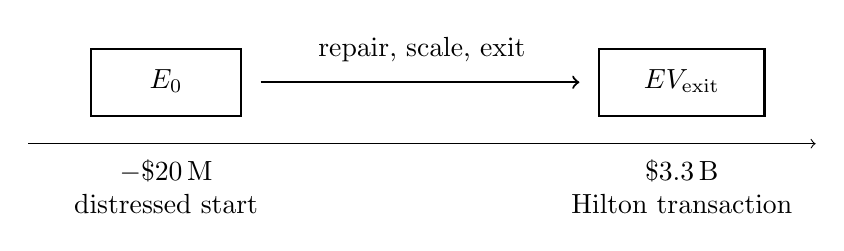
\begin{tikzpicture}[x=1cm,y=1cm]
\draw[->] (0,0) -- (10,0);
\draw[thick] (0.8,0.35) rectangle (2.7,1.2);
\node at (1.75,0.8) {$E_0$};
\node[align=center] at (1.75,-0.55) {$-\$20\,\mathrm{M}$\\distressed start};
\draw[->,thick] (2.95,0.78) -- (7.0,0.78);
\node at (5.0,1.2) {repair, scale, exit};
\draw[thick] (7.25,0.35) rectangle (9.35,1.2);
\node at (8.3,0.8) {$EV_{\mathrm{exit}}$};
\node[align=center] at (8.3,-0.55) {$\$3.3\,\mathrm{B}$\\Hilton transaction};
\end{tikzpicture}
\caption{A transcript-backed value ladder. The diagram is editorial, but the contrast it expresses is the opening arithmetic of the interview.}
\end{figure}

\section{Fixing Broken Systems: From Hospitality to Brand USA}

The second movement of the interview is a reframing. The speaker does not want to be heard merely as someone who sold a company. He wants to be heard as someone who fixes broken systems. This is why the lecture moves so quickly from the Hilton exit to Brand USA, tourism, public service, and a repeated insistence that the real work is to make everyone else look good.

That point is more technical than it first appears. The lecture is shifting the unit of analysis. If we speak only of the exit, then we are studying a terminal price. If we speak of fixing broken systems, then we are studying the operating path that makes such prices possible. The speaker's language is consistent: no trophies, no red carpet, no pride of authorship, only sleeves rolled up and work done.

When he says that the return on investment in Brand USA was ``outsized,'' the standard object is
\begin{equation}
\mathrm{ROI}=\frac{\text{incremental gain}-\text{cost}}{\text{cost}}.
\end{equation}
The interview supplies no numerical inputs for this expression, so we do not compute it. Still, the formula is useful because it clarifies the type of claim being made. The point is not ceremonial success. The point is that the intervention produced a large ratio of gain to cost.

The rest of the section broadens the same service ethic. He thought he might become a surgeon; instead he moved through shopping centers, hotels, politics, and policy. One phrase in the transcript is garbled, but the meaning is clear enough: service is not confined to executive altitude. The speaker wants to be legible from the lowest task to the highest room. That theme will return later with much greater force.

\paragraph{A first operational principle.}
The lecture quietly introduces its first durable principle here: value is built when institutions, customers, and counterparties are made to function better together. We are still near the beginning, but the chapter already refuses the fantasy of wealth without operations.

\section{Building the First Hotel Without Knowing How}

The lecture now narrows from scale to apprenticeship. The host asks about the first hotel, Polo Towers in Las Vegas, and the answer is not a clean origin story. It is an inventory of things not yet known. The speaker says he had built shopping centers, not hotels; then he describes a shopping-center project that went wrong in nearly every imaginable way. Contractors went broke. Lumber was paid for twice. Lien releases were not understood. Tenants failed. The economy was collapsing. A retaining wall, not present on the plans, suddenly had to be built at great expense.

This passage matters because it explains where later fluency comes from. The lecture does not romanticize ignorance. It presents ignorance as expensive. The speaker survives not by denying the cost of not knowing, but by learning under the pressure of it. He loses the shopping center but does not go broke. That distinction is central: survival preserves the right to learn again.

He then states the next milestone in the bluntest possible form:
\begin{equation}
a_{\mathrm{Polo}}\approx 29.
\end{equation}
At roughly that age, he says, he designed and built Polo Towers, which he describes as the largest hotel-timeshare complex ever built at one time in the world. We keep that as a speaker claim. What matters analytically is the sequence: technical ignorance, forced learning, survival, then execution.

\subsection{Question \& Answer}

\paragraph{Question.}
How do we build something we do not yet know how to build?

\paragraph{Answer.}
The lecture's answer is not mystical. It is cumulative.
\begin{enumerate}
\item We allow prior failure to become training rather than final identity.
\item We learn the actual object: how to read plans, how costs arise, where unseen liabilities hide.
\item We borrow standards from people who already know the terrain.
\item We remain close enough to the work that ignorance is corrected by contact rather than by abstraction.
\end{enumerate}
What the lecture rejects is the idea that courage can replace diligence. Courage is needed, but it is needed mainly to stay in the room long enough for diligence to work.

The account ends with an achievement that is almost classical in its terseness: on time, on budget, and done with his father. The lecture does not linger there. It immediately asks the next question, which is the right one. Once we have built the thing, how do we make it fit its customer?

\section{Customer, Naming, and the Early Brand Problem}

The next turn in the lecture is subtle but exact. The speaker says that he always kept things fresh and always listened to the customer. This is not a generic slogan. It is used to explain a specific design decision. The project carries the word ``Polo,'' a name with aristocratic overtones, but the target customer is broad. The speaker therefore says that he did not want the project to feel uncomfortable to the customer. It would not have the staid old English look one might expect; it would be modern.

This is the first mature appearance of brand in the interview. Brand begins here neither as advertising nor as self-expression. It begins as a constraint relation between a name, a target customer, and a felt environment. The project must signify distinction without pushing the customer away.

The trademark dispute with Ralph Lauren sharpens the point. The lecture presents the name not as decoration but as an asset worth defending. The argument is concrete: the mark was secured for hotel, timeshare, and casino use; the fight was costly; the name was retained. The sequence matters. First comes customer fit. Then comes legal protection. Only then do trademarks and domains appear in the lecture as serious objects.

The host then inserts a brief mentorship interlude before the interview resumes in another room. It is worth noting only because the rhythm changes when the conversation returns. Up to this point, the chapter has been mainly about the outer construction of a business. The next part will ask about the inner construction of the operator.

A final point closes the section. The speaker recalls that \emph{Undercover Boss} helped rather than harmed his brand, because it forced listening. The conclusion is stated plainly and should remain plain in the notes: it is not what we think or what the company thinks that finally decides the brand. It is what the customer thinks.

\section{Presence, Brand, and Leadership Under Pressure}

A visible object in the room, Iron Man, becomes the hinge for the next movement of the lecture. The speaker tells the story of being hit by a car, surviving, healing quickly, and acquiring the nicknames Iron Man and Wolverine. But the narrative point is not toughness for its own sake. The point is the maxim that follows: stay present. The lecture uses adversity to motivate attention. If we live in the past, we become depressed; if we live in the future, we become anxious; if we stay present, we can listen. And the lecture immediately adds the operational consequence: opportunity presents itself when we are actually attending to the person in front of us.

From there the interview passes directly into brand in its mature form. Brand is now treated as accumulated trust. To make that structure explicit, we introduce a cautious bookkeeping device:
\begin{definition}
Let \(B_t\) denote the stock of brand trust at time \(t\). It is not merely publicity. It is the accumulated memory of conduct, discipline, and respect.
\end{definition}

The lecture's verbal asymmetry can then be written as
\begin{equation}
B_{t+1}=B_t+\Delta B_t,
\end{equation}
with the important caution that the increments are not symmetric:
\begin{equation}
\Delta B_t^{+}\ \text{is slow and cumulative},\qquad
\Delta B_t^{-}\ \text{can be large and immediate}.
\end{equation}
This is the mathematical form of the claim that brand takes decades to build and minutes to kill.

\begin{figure}[h]
\centering
\begin{tikzpicture}[x=1cm,y=1cm]
\draw[->] (0,0) -- (10,0);
\draw[->] (0,0) -- (0,4.2);
\node at (9.5,-0.35) {time};
\node[rotate=90] at (-0.45,3.4) {brand trust};
\draw[thick] (0.6,0.45) -- (2.0,0.9) -- (3.8,1.6) -- (5.6,2.3) -- (7.6,3.1);
\draw[thick] (7.6,3.1) -- (8.35,0.9);
\node at (4.2,2.7) {slow build};
\node at (8.6,2.4) {trust break};
\end{tikzpicture}
\caption{A cautious reconstruction of the lecture's central asymmetry: brand accumulates slowly and can be destroyed quickly.}
\end{figure}

\subsection{Question \& Answer}

\paragraph{Question.}
If brand takes decades to build and minutes to kill, what exactly is being accumulated, and why can a single decision damage it so quickly?

\paragraph{Answer.}
What accumulates is not logo recognition by itself. It is remembered reliability. The lecture names its components again and again: integrity, discipline, respect, and a pattern of giving the customer a little more than was bargained for. A single lie can damage this stock quickly because one act can reveal the governing rule of a system. If the governing rule turns out to be deception, customers and colleagues update all previous signals at once.

This is why the lecture immediately moves to one of its hardest claims. The speaker says he had to fire the number one salesperson in the world because that person created a cancer in the organization. Everyone told him not to do it. He did it anyway. The result, he says, was
\begin{equation}
g_{\mathrm{post\text{-}removal}}\approx 20\%.
\end{equation}
We keep that as a speaker-attributed performance claim, not a causal proof. But the logic is crisp. If a star performer trains the system to violate its own brand, then short-run revenue may be buying long-run rot. Leadership, in this frame, is the willingness to prefer the integrity of the machine over dependence on a single producer.

\section{Speedboat Against Battleship: Founder Control Across the Operating Chain}

The lecture now asks how brand and discipline are made operational. The speaker says that he went around to great hotels, studied what worked and what did not, and compared Four Seasons, Ritz-Carlton, and Marriott. This is due diligence in the strict sense: comparison before imitation, and comparison in search of the space left open by incumbents.

What space was left open? The lecture's answer is not that the major firms were bad. It is that they had become too corporate, too rule-bound, too far from the entrepreneurial founder who speaks directly to the guest and can even write the front-desk script. From that point the lecture offers one of its best images:
\begin{equation}
R_{\mathrm{founder\text{-}led}} > R_{\mathrm{bureaucratic}},
\end{equation}
where \(R\) denotes responsiveness. This is not an econometric estimate. It is a compact way to formalize the speaker's verbal image of a battleship that can move like a speedboat.

\begin{figure}[h]
\centering
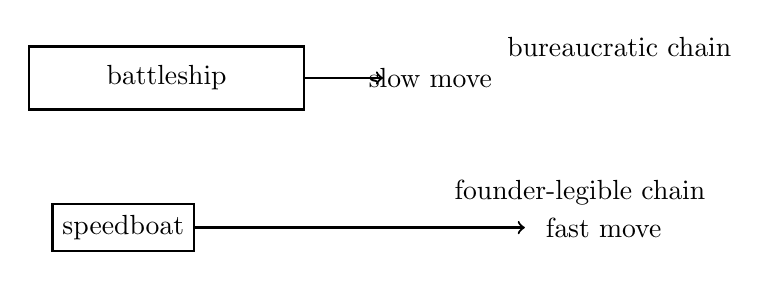
\begin{tikzpicture}[x=1cm,y=1cm]
\draw[thick] (0.5,2.5) rectangle (4.0,3.3);
\node at (2.25,2.9) {battleship};
\draw[->,thick] (4.0,2.9) -- (5.0,2.9);
\node at (5.6,2.9) {slow move};

\draw[thick] (0.8,0.7) rectangle (2.6,1.3);
\node at (1.7,1.0) {speedboat};
\draw[->,thick] (2.6,1.0) -- (6.8,1.0);
\node at (7.8,1.0) {fast move};

\node at (8.0,3.3) {bureaucratic chain};
\node at (7.5,1.45) {founder-legible chain};
\end{tikzpicture}
\caption{The lecture's image of corporate inertia and entrepreneurial speed. The point is not size alone, but the relation between decision rights and the work itself.}
\end{figure}

The chapter becomes highly concrete here, and it should remain concrete. The speaker says he could speak to any job in the business. He could write code for back-of-house systems, speak the language of tax accounting and facilities management, make a bed, specify towel placement, and even place a tent card under beds that said they had been cleaned there too. This is not mere performative humility. It is the operating grammar of the firm. The founder's legitimacy comes from demonstrated contact with every level of the machine.

\paragraph{Delegation in the lecture's sense.}
The interview does not reject delegation. It rejects blind delegation. One may coach, delegate, and scale, but only after making it visible that no task is outside the realm of understanding. That is why the speaker insists that there are no real titles in the deeper sense: only shared membership in the business and shared liability to the brand.

\section{Cashflow Shock, Bank Trust, Negotiation Silence, and the State as a Broken Business}

The chapter's last large movement begins with 9/11. The speaker is in the hotel business, flights are grounded, and guest flow vanishes. The lecture's arithmetic is now close to pure cashflow logic. If there are no guests, then operating inflow falls abruptly while obligations continue. A useful bookkeeping rule is
\begin{align}
C_{t+1} &= C_t + F_t + L_t - O_t,\\
F_t &\approx 0 \qquad \text{during the shutdown interval.}
\end{align}
Here \(C_t\) is cash, \(F_t\) is operating inflow, \(L_t\) is new liquidity obtained from lenders, and \(O_t\) is continuing obligation. The speaker says he called the banks every day, to the point that they asked him to call less often. The mathematical point is simple: when \(F_t\) collapses, survival cannot come from rhetoric. It comes from truthful communication and bridge liquidity.

\paragraph{A worked liquidity update.}
Suppose, purely as a bookkeeping example, that a firm enters the period with
\[
C_t=\$10\,\mathrm{M},\qquad O_t=\$6\,\mathrm{M},\qquad F_t=0,\qquad L_t=\$4\,\mathrm{M}.
\]
Then
\begin{align}
C_{t+1} &= C_t + F_t + L_t - O_t\\
&= \$10\,\mathrm{M}+0+\$4\,\mathrm{M}-\$6\,\mathrm{M}\\
&= \$8\,\mathrm{M}.
\end{align}
Nothing here is glamorous. That is exactly the point. The lecture treats crisis survival as disciplined arithmetic plus trustworthy communication.

\subsection{Question \& Answer}

\paragraph{Question.}
Why tell the bank the good, the bad, and the ugly instead of negotiating aggressively?

\paragraph{Answer.}
Because in the lecture's framework, future capital depends on trust before it depends on cleverness. The bank can price trouble if trouble is described honestly; it cannot price deception. Once trust is broken, forecasting becomes impossible. The lecture therefore prefers candor to theatrics.

This is the right place to record the three C's of banking as the speaker gives them:
\begin{itemize}
\item Capacity,
\item Character,
\item Credit.
\end{itemize}
The order is revealing. Character sits in the middle because the lecture insists that financial relationships are stabilized not only by numbers, but by repeated proof that the numbers will be discussed truthfully.

The negotiation doctrine that follows is consistent with this. The speaker says that the first person who talks loses, that one must not talk past the close, and that he once waited a week rather than breaking silence too soon. The operational sequence can be written schematically as
\begin{equation}
\text{close attempt} \longrightarrow \text{silence} \longrightarrow \text{counterparty movement}.
\end{equation}
Again, this is not a theorem. It is a disciplined heuristic. Its purpose is to resist the anxiety that tempts a seller to renegotiate against himself.

The lecture then makes its last scale change. After company, banks, and crisis, the same framework is applied to California. The speaker treats the state as a broken business rather than a conventional political abstraction. The two quantitative anchors he gives are
\begin{equation}
\operatorname{rank}_{\mathrm{GDP}}(\mathrm{California})=5,\qquad
N_{\mathrm{meetings}}>300.
\end{equation}
The first is a scale claim; the second is an input claim. He says California is effectively country-sized, that he met with more than three hundred people, and that the recurring failures were failures of customer communication, payroll understanding, execution, and regulatory balance.

The state-as-business analogy should be handled cautiously, but not dismissed. It is structurally continuous with the rest of the lecture. The same grammar is being reused:
\begin{itemize}
\item talk to the customer,
\item understand what payroll feels like,
\item distinguish necessary regulation from suffocating regulation,
\item execute,
\item tell the truth,
\item deliver results.
\end{itemize}
The lecture ends where it has been heading all along. A person who sees himself as a fixer of broken companies now sees the state as one more broken operating system.

\section{Summary}

The chapter begins with a startling contrast, \(E_0\approx -\$20\,\mathrm{M}\) and \(EV_{\mathrm{exit}}\approx \$3.3\,\mathrm{B}\), but the lecture does not allow that contrast to remain merely spectacular. It unpacks it. First come repair and institutional service; then apprenticeship under expensive error; then customer fit, naming, and trademark defense; then presence, brand, and hard leadership; then founder-legible operations; then crisis cashflow, bank trust, negotiation silence, and finally the scale-up from company to state.

What makes the lecture mathematically interesting is not formal abstraction for its own sake. It is the repeated conversion of biography into operational structure. Brand becomes an update rule. Crisis becomes a cash recurrence. Responsiveness becomes a relation between organizational form and decision speed. In that sense the interview's deepest claim is plain: large outcomes are not produced by a single heroic leap, but by a long sequence of disciplined updates that preserve trust while increasing scale.